\documentclass[numbers,10pt,preprint]{sigplanconf}
\usepackage{array}
\usepackage{fontspec}
\setmainfont[Ligatures=TeX]{Times New Roman}
\setmonofont{APL385 Unicode}
\usepackage{graphicx}
\usepackage[scaled]{helvet} % see www.ctan.org/get/macros/latex/required/psnfss/psnfss2e.pdf
\usepackage{url}                  % format URLs
\usepackage{listings}          % format code
\usepackage{enumitem}      % adjust spacing in enums
\usepackage[colorlinks=false,allcolors=blue,breaklinks,draft=false]{hyperref}   % hyperlinks, including DOIs and URLs in bibliography
% known bug: http://tex.stackexchange.com/questions/1522/pdfendlink-ended-up-in-different-nesting-level-than-pdfstartlink
\newcommand{\doi}[1]{doi:~\href{http://dx.doi.org/#1}{\Hurl{#1}}}   % print a hyperlinked DOI
\usepackage{booktabs}

\begin{document}

\title{The Key to a Performant Data Parallel Compiler}
\authorinfo{Aaron W. Hsu}{Indiana University, USA}{awhsu@indiana.edu}
\maketitle

\begin{abstract}
We present a language-driven strategy for the construction of compilers that are inherently data-parallel in their design and implementation. Using an encoding of the inter-node relationships between nodes in an AST called a Path Matrix, we demonstrate how an operator called the Key operator, that applies a function over groupings of array cells grouped and ordered by their keys, when used in conjunction with a Path Matrix, permits arbitrary computation over sub-trees of an AST using purely data-parallel array programming techniques. We discuss the use of these techniques when applied to an experimental commercial compiler called Co-dfns, a fully data-parallel compiler developed using the techniques discussed here. On transformation heavy operations such as expression flattening or function lifting, these techniques, when compared against pure and effectful recursive implementations, outperforms the CPU-based algorithms by a factor of 10 - 58 on the GPU. 
\end{abstract}

\category{D.3.4}{Programming Languages}{Processors}[Compilers]
\terms Algorithms, Performance, Design, Languages
\keywords APL, Parallel, Compilers, Key, Node Coordinates

\section{Introduction}

Compilers represent a peculiar class of tree/graph algorithms that greatly alter the underlying structure of the input graph into something very different in structure, but equivalent by some semantic interpretation. These algorithms are widely applicable, but have stubbornly resisted a general approach to parallelization. Most compilers are single-threaded or make very limited use of parallelism in an ad hoc way. The design and analysis of compilers almost universally deals with compilers as recursive traversals over ASTs. Such formulations usually include heavy reliance on branching, recursion, and sometimes very sophisticated control flow. All of this contributes to make it difficult to effectively parallelize such algo-rithms onto architectures that are sensitive to branching and recursion, such as GPGPUs or highly vectorised CPUs.

There has been some success in efficiently executing parts of a compiler on the GPU, such as the parser \cite{bunda1984apl}, tokenization \cite{bernecky2003tokenizer}, and certain compiler analyses \cite{prabhu2011eigencfa,mendez2012inclusion}. However, a generalized framework or strategy for parallel compilation remains elusive. One of the major difficulties is the recursive and highly branch dependent nature of the algorithms. These present challenges that must be overcome in vector-centric architectures.

We present a language-driven strategy for creating an inherently parallel compiler. We select a set of well known data-parallel primitives, and then restrict program construction to the composition of these operations into functions, without any forms of non-linear control flow, such as branching, recursion, or pattern matching. Programs constructed in such a style are data-parallel by construction. A key problem to the construction of compilers in such a restricted environment is dealing with the inherently recursive and nested structure of the AST. By working over a linearized representation of the AST as a matrix, combined with a structure we call a Path Matrix, and using data-parallel primitives, we are able to tame the recursive and nested nature of the AST into something that can be processed handily using only data-parallel, data-flow programs, without requiring branching or other forms of non-data parallel control flow. The methods are general and independent of the language being compiled.

In the following sections we describe the core methods and idioms surrounding the AST encoding, construction of the Path Matrix, and the use of these structures in handling nested, recursive AST relationships. This enables us to perform arbitrary computation over arbitrary sub-trees of an AST selected by parent-child relationships in the manner often seen in compiler transformations. These ideas have been further implemented and tested through the implementation of a complete data-parallel by construction compiler, called Co-dfns, that compiles a lexically scoped, functionally oriented dialect of APL with nested functions \cite{hsu2014co,hsu2015accelerating}. The compiler targets both the GPU and the CPU, and its core is implemented in this pure, restricted language that uses only function composition over data-parallel primitives.

To illustrate the performance of these techniques, we micro-benchmark a transformation heavy expression lifting algorithm that is found almost universally in compilers. This benchmark shows performance speedups of up to a factor of 58 when compared against pure, functionally oriented algorithms.

\paragraph{Contributions}

\begin{itemize}[noitemsep]

\item We describe a method of computing over arbitrary sub-trees selected by their parent-child relationships in a data-parallel manner using the Key operator and a Path Matrix.

\item We situate this technique into a broader, language-driven strategy for compiler construction that enables the development of parallel by construction compilers that are high-level in their implementation, exceptionally concise, and independent of the language being compiled.

\item We provide analysis of these techniques as used in a commercial compiler project called Co-dfns and report on the results, including the overall architecture of the compiler, the uses of these techniques within the compiler, and the demonstration of these techniques applied to two specific compiler passes.

\item We compare the performance of the Key-based algorithms against traditional recursive methods for the task of lifting/flattening expressions, such as commonly done for function lifting and expression flattening. Our results demonstrate consistent speedups over the traditional methods.

\end{itemize}

\section{Notational Conventions}

For space and convenience, we use a concise array notational convention to describe our techniques and approach. The notation is executable and well established in the array community (it is a limited subset of APL). This is in fact the same notation used within the Co-dfns compiler itself, whose source code is available online and provides a complete example of the use of both these algorithms and this notation in the large. All code examples are given in the following form:

\begin{verbatim}
      5×3+4 ⍝ Right to Left Evaluation
35
\end{verbatim}

\noindent That is, we indent the expression by 6 spaces, followed by the value of the expression without indent. All expressions are evaluated right to left and all function application is infix; that is, a function application may apply a function (such as \verb;+;) to one or two arguments, called monadic and dyadic application respectively, which must appear on the right and (optionally) on the left of the function name, as in the above example. The Appendix provides a listing of all of the primitives used in the Co-dfns compiler, a selection of which are used here.

We differentiate higher-order functions called operators, from functions that operate over arrays that we call simply functions. Operators take a function argument or two, and bind more strongly to the left than the right. An operator may take one or two operands, either on the left, or on the right and left, and will return a function. In the following example, we apply the reduction operator (\verb;/;) to a function created using the composition operator (\verb;∘;), as an example:

\begin{verbatim}
      +/1 2 3 4 5
15
      1+-(2+-(3+-(4+-(5))))
3
      1 +∘- 2 +∘- 3 +∘- 4 +∘- 5
3
      +∘-/1 2 3 4 5
3
\end{verbatim}

\noindent We introduce notation as needed throughout the exposition, so the reader is encouraged to refer to the appendix as necessary to recall particular operations.

\section{Data Parallel Sub-tree Computation}

Computing over sub-trees normally involves recursing down the structure of the AST, identifying the root nodes of each sub-tree, and then dispatching to a handler for that sub-tree, which will continue the recursion at that point and return the modified tree, which will replace the previous sub-tree. More complicated transformations may involved moving the root nodes around in the tree or other large, distant structural modifications.

We divide the work of sub-tree computation into three basic phases: we maintain a node coordinate with each node that uniquely identifies it relative to others, we use these coordinates to select and group nodes for work as a single sub-tree, and then we operate over these groupings using the Key operator (\verb;⌸;).

\subsection{Encoding the AST}

We represent the AST as a 3 column matrix with one row per node in the tree. The first column contains the inter-node relationships in the form of a depth vector. The second column is a vector of the node types, while the third contains the ``value'' of the node, such as the name in a variable.

We will use the following two running examples throughout. The \verb;F; tree is an example nested function, while the \verb;E; tree is an example nested expression.

\begin{verbatim}
      F(f)              E(v)
       │         ┌───────┼──────┐
       E         E      P(÷)    E
     ┌─┴─┐  ┌────┼────┐    ┌────┼────┐
     F   A V(a) P(+) V(b) V(c) P(×) V(d)
     │   │
     E  N(7) 
 ┌───┼────┐
V(⍵) P(+) V(⍵)
\end{verbatim}

\noindent
The depth vectors for these trees we name \verb;Fd; and \verb;Ed;, respectively:

\begin{verbatim}
Fd←0 1 2 3 4 4 4 2 3
Ed←0 1 2 2 2 1 1 2 2 2
\end{verbatim}

\noindent
The node types we call \verb;Ft; and \verb;Et;:

\begin{verbatim}
Ft←'FEFEVPVAN'
Et←'EEVPVPEVPV'
\end{verbatim}

\noindent
And finally, we call the values vectors \verb;Fv; and \verb;Ev;:

\begin{verbatim}
Fv←'f' 0 0 0 '⍵' '+' '⍵' 0 7
Ev←'v' 0 'a' '+' 'b' '÷' 0 'c' '×' 'd'
\end{verbatim}

\noindent We combine these to form the respective AST matrices. We write \verb;A,B; to catenate arrays \verb;A; and \verb;B; along their last axes and \verb;⍪A; to turn a vector into a 1-column matrix. Thus, the two AST matrices are given by the following expressions:

\begin{verbatim}
      Fd,Ft,⍪Fv  │        Ed,Et,⍪Ev
0 F f            │  0 E v
1 E 0            │  1 E 0
2 F 0            │  2 V a
3 E 0            │  2 P +
4 V ⍵            │  2 V b
4 P +            │  1 P ÷
4 V ⍵            │  1 E 0
2 A 0            │  2 V c
3 N 7            │  2 P ×
                 │  2 V d
\end{verbatim}

\noindent The depth vector stores all edge information for the tree, but this information requires non-local access to utilize, such as traversing potentially the entire vector to determine the children of a specific node. Node Coordinates fix this issue.

\subsection{Node Coordinates}

Every node in an AST has a Node Coordinate, named because a coordinate is a precise location in a space.  We can imagine all the nodes arranged inside some multi-dimensional space, leading to a specific set of node coordinates. Many such arrangements exist, of varying usefulness. In our case, any arrangement should allow us to answer the following questions about any two arbitrary nodes in a tree:

\begin{enumerate}[noitemsep]
\item Are the nodes the same?
\item Are they siblings?
\item Does one appear ``earlier'' in the tree?
\item Are they at the same depth?
\item Is one an ancestor of another?
\end{enumerate}

\noindent In short, we care about the relative position of each node in a tree relative to any other. We define a node coordinate as follows.

A node coordinate is a vector whose length is the depth of the tree. Its elements are natural numbers.  The count of non-zero elements in the vector is equal to the depth of that node in the tree. All zero elements appear after the non-zero elements. That is, a coordinate is zero-padded on the right. When ordered lexicographically, the nodes for each coordinate appear in order according to a depth-first pre-order traversal of the tree. Each coordinate uniquely identifies a single node. Every ancestor’s coordinate is a prefix of any child’s coordinate, ignoring zeros. From the above it follows that every node is lexicographically greater than its left sibling and differs from it by exactly one non-zero element, and that this element is the last non-zero element in the coordinate.

\subsubsection{Constructing Node Coordinates}

We construct the Node Coordinate Matrix from the depth vector, thereby encoding the depth vector into a more useful format. The matrix has \verb;N; rows and \verb;D; columns, where \verb;N; is the node count and \verb;D; is the depth of the tree.

We write \verb;f⌿A; to reduce the first axis of \verb;A; using function \verb;f;. Thus, \verb;+⌿V; is the sum of the elements in vector \verb;V;. The function \verb;x⌈y; gives the maximum of its two arguments. We compute the depth of each tree as follows:

\begin{verbatim}
      1+⌈⌿Fd  │        1+⌈⌿Ed
5             │  3
\end{verbatim}

\noindent We can obtain the ordered sequence  by writing \verb;⍳n;:

\begin{verbatim}
      ⍳3
0 1 2
\end{verbatim}

\noindent
So the depths of all nodes that appear in the depth vectors is thus:

\begin{verbatim}
      ⍳1+⌈⌿Fd │        ⍳1+⌈⌿Ed
0 1 2 3 4 5   │  0 1 2
\end{verbatim}

\noindent The function table or outer product of \verb;f; over vectors \verb;U; and \verb;V; is written \verb;U ∘.f V; giving a \verb;U V; shaped matrix as a result. Thus, \verb;(⍳3)∘.×⍳3; gives a small multiplication table:

\begin{verbatim}
      (⍳3)∘.×⍳3  │        ⍳3
0 0 0            │  0 1 2
0 1 2            │        ⍴⍳3
0 2 4            │  3
\end{verbatim}

\noindent If we use \verb;=; instead, we have a Boolean identity matrix:

\begin{verbatim}
      (⍳3)∘.=⍳3
1 0 0
0 1 0
0 0 1
\end{verbatim}

\noindent If we use \verb;∘.=; on the depth vector and its set of depths instead, we see an expanded Boolean representation of the depth vector:

\begin{verbatim}
      Fd∘.=⍳1+⌈⌿Fd │      Ed∘.=⍳1+⌈⌿Ed
1 0 0 0 0          │ 1 0 0
0 1 0 0 0          │ 0 1 0
0 0 1 0 0          │ 0 0 1
0 0 0 1 0          │ 0 0 1
0 0 0 0 1          │ 0 0 1
0 0 0 0 1          │ 0 1 0
0 0 0 0 1          │ 0 1 0
0 0 1 0 0          │ 0 0 1
0 0 0 1 0          │ 0 0 1
                   │ 0 0 1
\end{verbatim}

\noindent These matrices let us see the nesting features of each tree more visually, but also suggest another step. We can compute a sum scan with \verb;+⍀;, also called a prefix sum, along the first axis. Applying this function on the above matrices leads to an interesting result:

\begin{verbatim}
    +⍀Fd∘.=⍳1+⌈⌿Fd  │     +⍀Ed∘.=⍳1+⌈⌿Ed
1 0 0 0 0           │ 1 0 0
1 1 0 0 0           │ 1 1 0
1 1 1 0 0           │ 1 1 1
1 1 1 1 0           │ 1 1 2
1 1 1 1 1           │ 1 1 3
1 1 1 1 2           │ 1 2 3
1 1 1 1 3           │ 1 3 3
1 1 2 1 3           │ 1 3 4
1 1 2 2 3           │ 1 3 5
                    │ 1 3 6
\end{verbatim}

\noindent These matrices are lexicographically ordered, and each ancestor shares a common prefix with its descendants. They are also unique coordinates. Only the spurious digits at the end of each coordinate prevent these matrices from meeting all our requirements for valid node coordinates.

The expression \verb;V f⍤¯1⊢M; applies \verb;f; to corresponding elements of \verb;V; and rows of \verb;M;:

\begin{verbatim}
      3 3⍴⍳9 │       (⍳3)+⍤¯1⊢3 3⍴⍳9
0 1 2        │ 0 1  2
3 4 5        │ 4 5  6
6 7 8        │ 8 9 10
\end{verbatim}

\noindent If \verb;n↑V; takes the first \verb;n; elements of \verb;V;, then we can obtain coordinate matrices from the prefix sums by noting that the spurious digits all come after column \verb;d+1; where \verb;d; is the depth corresponding to that coordinate. The following gives a complete expression for computing a node coordinate matrix from a depth vector, shown using \verb;Fd; and \verb;Fe;:

\begin{verbatim}
      Fc←(1+Fd)↑⍤¯1⊢+⍀Fd∘.=⍳1+⌈⌿Fd
      Ec←(1+Ed)↑⍤¯1⊢+⍀Ed∘.=⍳1+⌈⌿Ed
      Fc   │        Ec
1 0 0 0 0  │  1 0 0
1 1 0 0 0  │  1 1 0
1 1 1 0 0  │  1 1 1
1 1 1 1 0  │  1 1 2
1 1 1 1 1  │  1 1 3
1 1 1 1 2  │  1 2 0
1 1 1 1 3  │  1 3 0
1 1 2 0 0  │  1 3 4
1 1 2 2 0  │  1 3 5
           │  1 3 6
\end{verbatim}

A careful study of the definition of a node coordinate and the above construction should reveal why this works. Intuitively, we are creating a multi-dimensional space or a number system in which each digit place or dimension contains or circumscribes a smaller space in which are contained all the descendant nodes that appear lower in the tree. Each coordinate is a sort of special path through the tree encoded to have desirable properties relative to other paths.

\subsubsection{Operations on Node Coordinates}

The simplest operation over a node coordinate is to extract the depth of the node. The dyadic expression \verb;C⍳0; finds the first occurrence of \verb;0; in \verb;C; and returns the index of that occurrence. Thus, we compute the depth of a node as follows:

\begin{verbatim}
      C←1 1 2 0 0
      ¯1+C⍳0
2
\end{verbatim}

\noindent In many compiler passes, we primarily care about which nodes are ancestors of other nodes. To determine whether one node is a child of another, we compute whether one node is a prefix of the other, ignoring zeros. We write \verb;(f g h); to represent the composition of functions \verb;f;, \verb;g;, and \verb;h; as a function train. Function trains obey the following equivalences, where \verb;A; and \verb;B; are arrays.

\begin{verbatim}
A(f g h)B ←→ (A f B) g (A h B)
A(0 f h)B ←→ 0 f (A h B) ⍝ Constant Case
A(f g)B   ←→ f (A g B)
\end{verbatim}

\noindent With this, we write a function to compute whether a given coordinate prefixes another.

\begin{verbatim}
      P←1 1 0 0 0
      C(=∨0=⊢)P
1 1 1 1 1
      ∧⌿C(=∨0=⊢)P
1
\end{verbatim}

\noindent The above determines whether \verb;P; is an ancestor to \verb;C;. The logical functions \verb;=;, \verb;∧;, and \verb;∨; are all extended point-wise over arrays. The function \verb;⊢; returns its right argument. The function \verb;(=∨0=⊢); reads as, ``equal or a zero right argument.'' We take this point-wise operation and reduce it with \verb;∧⌿; (For All). This pattern is a special case of inner product, written \verb;f.g;. For example, \verb;+.×; is matrix multiplication. We transform our reduction and Boolean function to a single predicate with the inner product operator:

\begin{verbatim}
      C∧.(=∨0=⊢)P
1
\end{verbatim}

The use of inner product extends to cases where \verb;C; or \verb;P; are matrices. For our examples, we want to lift the functions and flatten expressions, so we will select the \verb;F; nodes and \verb;E; nodes, respectively, as our parent/ancestor nodes in \verb;Fp; and \verb;Ep;. Given a boolean vector \verb;BV;, the expression \verb;BV⌿M; selects rows from \verb;M; based on the non-zero elements of \verb;BV;.

\begin{verbatim}
      Fp←('F'=Ft)⌿Fc
      Ep←('E'=Et)⌿Ec
      Fp   │        Ep
1 0 0 0 0  │  1 0 0
1 1 1 0 0  │  1 1 0
           │  1 3 0
\end{verbatim}

\noindent We could use \verb;Fp; and \verb;Ep; to compare against \verb;Fc; and \verb;Ec; to determine which nodes belong to which parent in \verb;Fp; or \verb;Ep;, but our prefix function returns 1 when \verb;C≡P;. Instead, we drop the last non-zero element from each coordinate. This will permit matching against all ancestors, but not against itself. We use the depth vector and the Take (\verb;↑;) function to take all but the last non-zero element. We extend the resulting array with an extra zero column to ensure we have a compatible shape.

\begin{verbatim}
      Fcp←(Fd↑⍤¯1⊢Fc),0
      Ecp←(Ed↑⍤¯1⊢Ec),0
      Fcp  │        Ecp
0 0 0 0 0  │  0 0 0
1 0 0 0 0  │  1 0 0
1 1 0 0 0  │  1 1 0
1 1 1 0 0  │  1 1 0
1 1 1 1 0  │  1 1 0
1 1 1 1 0  │  1 0 0
1 1 1 1 0  │  1 0 0
1 1 0 0 0  │  1 3 0
1 1 2 0 0  │  1 3 0
           │  1 3 0
\end{verbatim}

\noindent We use \verb;Fcp; and \verb;Ecp; to determine the \verb;F; and \verb;E; ancestors for each node (\verb;⍉A; transposes \verb;A;):

\begin{verbatim}
   Fcp∧.(=∨0=⊢)⍉Fp │    Ecp∧.(=∨0=⊢)⍉Ep
0 0                │ 0 0 0
1 0                │ 1 0 0
1 0                │ 1 1 0
1 1                │ 1 1 0
1 1                │ 1 1 0
1 1                │ 1 0 0
1 1                │ 1 0 0
1 0                │ 1 0 1
1 0                │ 1 0 1
                   │ 1 0 1
\end{verbatim}

\noindent In the above, the closest ancestor is the rightmost 1 in each row. We can extract the column number of the rightmost 1 by replacing each 1 with its column number and selecting the maximum of each row with \verb;⌈/;. For space we will show only the \verb;E; example. In the following, \verb;V×⍤1⊢M; gives a matrix where each row is given by \verb;V×i⌷M; where \verb;i⌷M; is the $i$th row of \verb;M;.

\begin{verbatim}
      (⍳3)×⍤1⊢Ecp∧.(=∨0=⊢)⍉Ep
0 0 0
0 0 0
0 1 0
0 1 0
0 1 0
0 0 0
0 0 0
0 0 2
0 0 2
0 0 2
      ⊢Ei←⌈/(⍳3)×⍤1⊢Ecp∧.(=∨0=⊢)⍉Ep
0 0 1 1 1 0 0 2 2 2
      ⊢Fi←⌈/(⍳2)×⍤1⊢Fcp∧.(=∨0=⊢)⍉Fp
0 0 0 1 1 1 1 0 0
\end{verbatim}

\noindent We use these column numbers to index into \verb;Ep; to obtain an ancestor matrix where the node coordinate of the closest ancestor is given for each node, one per row. The expression \verb;I⌷⍤0 2⊢M; gives a matrix, one row per index in \verb;I;, consisting of rows of \verb;M; selected by row indices in \verb;I;.

\begin{verbatim}
      Fk←Fi⌷⍤0 2⊢Fp
      Ek←Ei⌷⍤0 2⊢Ep 
      Fk   │        Ek
1 0 0 0 0  │  1 0 0
1 0 0 0 0  │  1 0 0
1 0 0 0 0  │  1 1 0
1 1 1 0 0  │  1 1 0
1 1 1 0 0  │  1 1 0
1 1 1 0 0  │  1 0 0
1 1 1 0 0  │  1 0 0
1 0 0 0 0  │  1 3 0
1 0 0 0 0  │  1 3 0
           │  1 3 0
\end{verbatim}

\noindent At this point we have two values, \verb;Ek; and \verb;Fk;, which indicate the closest containing node that we care about for each node in the tree, using its node coordinate. We use these keys to compute over the AST, particularly for function lifting and expression flattening as demonstrated in the next section. The repeating pattern is to leverage node coordinates and array operations to do stackless reasoning about inter-node relationships. This pattern occurs often in our compiler and is particularly useful to enable straightforward data-parallel transformations over an AST.

\begin{table*}
\centering
\begin{tabular}{l p{2.8in} l l l}
\toprule
Pass & Description & Core Traversal Pattern & Uses coordinates? \\
\midrule
Record Node Coordinates & Adds a new field to each node containing that node's 
 node coordinate. & Outer Product/Scan & Yes \\
Record Function Depths & Adds a new field to each node recording how many 
 functions surround the node. & Inner Product & Yes \\
Drop Unnamed Functions & Eliminates some code that will not be evaluated at 
 the top-level. & Filter & No \\
Drop Unreachable Code & Eliminates some unreachable code. &
 Filter/Inner Product & Yes \\
Lift Functions & Moves all functions to the top-level. & Key & Yes \\
Drop Redundant Nodes & Eliminates unnecessary nodes/nesting. & Filter & No \\
Flatten Expressions & Removes nesting from expressions. & Key & Yes \\
Compress Atomic Nodes & Atomizes nested atom nodes. & Amend & No \\
Propagate Constants & Inlines all references to literal values. &
 Amend/Rank & Yes \\
Fold Constants & Converts constant expressions to literals. & Amend & No \\
Compress Expressions & Converts expression sub-trees into single nodes. & 
 Amend & No \\
Record Final Return Value & Records the value returned by each function. & 
 Key & No \\
Normalize Values Field & Normalizes the shape and size of the values field. &
 Amend & No \\
Lift Type-checking & Infers some type information at compile time. &
 Power Limit/Rank & No \\
Allocate Value Slots & Does a form of frame allocation for variables. &
 Key & No \\
Anchor Variables & Resolves lexically scoped variables. &
 Key & Yes \\
Record Live Variables & Records the variables that are live at each point of 
 execution. & Key & No \\
Fuse Scalar Loops & Identifies Fusion opportunities and fuses expressions. &
 Key & No \\
Type Specialization & Specializes each function for a series of potential inputs. 
 & Key & No \\
\end{tabular}
\caption{A listing of some compiler passes in the Co-dfns compiler and their 
 relationship with the Key operator and associated tree computation techniques}
\label{tab:passes}
\end{table*}

\subsection{The Key Operator}

First introduced in the J language \cite{hui2014key}, the Key operator (written \verb;⌸;) is central to our strategy for compilation. It allows us to use the Node Coordinates to their full effect. The expression \verb;K f⌸ M; groups rows of \verb;M; by their corresponding keys in \verb;K; and computes \verb;k f m; for each unique key \verb;k; in \verb;K; and the matrix \verb;m; of rows of \verb;M; with key \verb;k;. The corresponding rows of matrices \verb;K; and \verb;M; form key-value pairs. Let's compute a histogram using Tally (\verb;≢;) and Key (\verb;⌸;):

\begin{verbatim}
      10⍴5
5 5 5 5 5 5 5 5 5 5
      ⊢X←?10⍴5
1 1 4 0 1 3 1 1 2 1
      ≢⍳5
5
      X(⊣,(≢⊢))⌸X
1 6
4 1
0 1
3 1
2 1
\end{verbatim}

\noindent To understand a bit better how the Key operator applies its function, consider the function \verb;{⍺ ⍵}; which returns the pair of its right and left arguments. If we apply it to the same value as above, we get the following:

\begin{verbatim}
      X{⍺ ⍵}⌸X
1  1 1 1 1 1 1 
4  4           
0  0           
3  3           
2  2
\end{verbatim}

\noindent In our case, we use either \verb;Fk; or \verb;Ek; as our keys applied to the corresponding AST. We also will drop off the first row in each AST using \verb;1↓; since this node ``contains'' everything. In a complete AST this is usually the Module boundary node which contains the entire set of functions and values in the module.

\section{Case Studies}

The following compiler passes are found in any compiler from a nested function, nested expression language to a language without nested functions or expressions. They were the chief motivating examples for developing the techniques presented above as a part of developing the Co-dfns compiler, and represent a challenging problem to data-parallel compilation without the above techniques, but fall out almost effortlessly once the above patterns are available.

Each of the following passes operates over an AST that we represent as the catenation of the field vectors above including the Node Coordinates.

\begin{verbatim}
Fast←Fd,Ft,Fv,⍪↓Fc
East←Ed,Et,Ev,⍪↓Ec
\end{verbatim}

\noindent The function \verb;↓; converts the coordinate matrices from matrices to vectors of vectors, so that the coordinates can be catenated to the other fields, leading to a 4-column matrix for the ASTs, whose fourth column is a vector of vectors. 

\subsection{Function Lifting}

Function lifting takes an AST with nested functions (func-tions appearing inside of other functions) and lifts these functions out of their local scopes and puts them all at the top level. Normally, function lifting must consider both the core operation of lifting function as well as the lexical scop-ing of the functions and variables that appear inside of a function. As seen below, our treatment uses a slightly dif-ferent method. 

If we use the Key operator (\verb;⌸;) with the pair function (\verb;{⍺ ⍵};) using \verb;Fk; as the keys and \verb;Fast; as the AST, we get the following:

\begin{verbatim}
      (1↓Fk){⍺ ⍵}⌸1↓Fast
┌─────────┬─────────────────┐
│1 0 0 0 0│┌─┬─┬─┬─────────┐│
│         ││1│E│0│1 1 0 0 0││
│         │├─┼─┼─┼─────────┤│
│         ││2│F│0│1 1 1 0 0││
│         │├─┼─┼─┼─────────┤│
│         ││2│A│0│1 1 2 0 0││
│         │├─┼─┼─┼─────────┤│
│         ││3│N│7│1 1 2 2 0││
│         │└─┴─┴─┴─────────┘│
├─────────┼─────────────────┤
│1 1 1 0 0│┌─┬─┬─┬─────────┐│
│         ││3│E│0│1 1 1 1 0││
│         │├─┼─┼─┼─────────┤│
│         ││4│V│⍵│1 1 1 1 1││
│         │├─┼─┼─┼─────────┤│
│         ││4│P│+│1 1 1 1 2││
│         │├─┼─┼─┼─────────┤│
│         ││4│V│⍵│1 1 1 1 3││
│         │└─┴─┴─┴─────────┘│
└─────────┴─────────────────┘
\end{verbatim}

Notice that we have now grouped all of the relevant parts of the tree according to which nodes would appear in their respective functions after lifting. Refer to the original lifting example in the introduction to verify this. Indeed, the second row in the above example shows the internal function complete and ready to name. Each element in the second column corresponds to the body of one of our lifted functions. In the case of the first function, the outer function, we have a spurious function node in the body. This is intentional. When we lift these functions, we will replace each spurious function node with a variable node referring to the function’s generated name.

Each of these grouped sub-trees will be given a new local root \verb;F; node that is at the appropriate depth (0) and uses the key as its path vector (\verb;⊣;).

\begin{verbatim}
      (1↓Fk){⊂(0 'F' 0 ⍺)⍪⍵}⌸1↓Fast
┌─────────────────┬─────────────────┐
│┌─┬─┬─┬─────────┐│┌─┬─┬─┬─────────┐│
││0│F│0│1 0 0 0 0│││0│F│0│1 1 1 0 0││
│├─┼─┼─┼─────────┤│├─┼─┼─┼─────────┤│
││1│E│0│1 1 0 0 0│││3│E│0│1 1 1 1 0││
│├─┼─┼─┼─────────┤│├─┼─┼─┼─────────┤│
││2│F│0│1 1 1 0 0│││4│V│⍵│1 1 1 1 1││
│├─┼─┼─┼─────────┤│├─┼─┼─┼─────────┤│
││2│A│0│1 1 2 0 0│││4│P│+│1 1 1 1 2││
│├─┼─┼─┼─────────┤│├─┼─┼─┼─────────┤│
││3│N│7│1 1 2 2 0│││4│V│⍵│1 1 1 1 3││
│└─┴─┴─┴─────────┘│└─┴─┴─┴─────────┘│
└─────────────────┴─────────────────┘ 
\end{verbatim}

\noindent At this point, the internal function nodes refer by path vector to the newly added local roots. This was down without traversing or maintaining these connections, but falls out as a natural artifact of using the Key (\verb;⌸;) operator. At this point we are ready to fix up the sub-tree to be correct. Firstly, we need a function to encapsulate the function header information.

\begin{verbatim}
      hd←0 'F' 0,∘⊂⊣      ⍝ Func. Header
\end{verbatim}

\noindent Next, we write a function to adjust the depths, which is one more than the difference between each node's depth and the depth of the first node of the sub-tree. 

\begin{verbatim}
      dp←(1+⊢-⊃)0⌷⍤1⊢     ⍝ New Depths
\end{verbatim}

\noindent Finally, we use the \verb;@; operator to replace occurances of \verb;F; in the Type column with \verb;V; elements. 

\begin{verbatim}
      rf←'V'@('F'∘=)1⌷⍤1⊢ ⍝ F → V
\end{verbatim}

\noindent Once we put all this together, we can construct the new sub-trees with the appropriate depths, types, references, and links with the following expression.

\begin{verbatim}
      (1↓Fk)(⊂hd⍪dp,rf,2↓⍤1⊢)⌸1↓Fast
┌─────────────────┬─────────────────┐
│┌─┬─┬─┬─────────┐│┌─┬─┬─┬─────────┐│
││0│F│0│1 0 0 0 0│││0│F│0│1 1 1 0 0││
│├─┼─┼─┼─────────┤│├─┼─┼─┼─────────┤│
││1│E│0│1 1 0 0 0│││1│E│0│1 1 1 1 0││
│├─┼─┼─┼─────────┤│├─┼─┼─┼─────────┤│
││2│V│0│1 1 1 0 0│││2│V│⍵│1 1 1 1 1││
│├─┼─┼─┼─────────┤│├─┼─┼─┼─────────┤│
││2│A│0│1 1 2 0 0│││2│P│+│1 1 1 1 2││
│├─┼─┼─┼─────────┤│├─┼─┼─┼─────────┤│
││3│N│7│1 1 2 2 0│││2│V│⍵│1 1 1 1 3││
│└─┴─┴─┴─────────┘│└─┴─┴─┴─────────┘│
└─────────────────┴─────────────────┘
\end{verbatim}

Each of these function bodies has a specific coordinate associated with it. Because these coordinates are uniquely identifying, we can use these as input into a name generator to generate names that we know are unique for each function body. Furthermore, because we retain this information in the corresponding function nodes that appear in the body of each function to be lifted, we know exactly what name that function has been given, and we can replace the function node with a variable node referencing that name instead, without referring to any state outside of the immediate information given to the function lifter. Indeed, each row in the above matrix represents a function lifting task that can be completed without any additional information. That is, there are no dependencies between rows to perform lifting. This gives us a straightforward parallel execution of function lifting.

This function lifting works even with lexically scoped functions, as is the case for the Co-dfns compiler. We can do this because the node coordinates maintain the lexical information for each variable reference, enabling us to construct the appropriate lexical binding for each variable much later than would normally be done in a compiler. In other words, the above lifting operation loses no information that would prevent us from handling lexical scoping, but decouples lexical scoping from the act of lifting functions.

\subsection{Expression Flattening}

Flattening expressions is almost identical to lifting functions, in part because we have delayed the lexical scope resolution aspect of lifting functions to a later pass that will handle this explicitly. In addition to lifting the expressions themselves, however, we will also take the opportunity to handle precedence and ordering. In our examples, we are assuming that all expressions evaluate right to left. Because the Key (\verb;⌸;) operator is a stable operation, and we require that nodes have a depth-first pre-order traversal pattern, then we can trivially handle precedence order of this type, including handling parentheses, by reversing the results of flattening.

If we use \verb;Ek; as the key for the expression example, we get the following:

\begin{verbatim}
      (1↓Ek){⍺ ⍵}⌸1↓East
┌─────┬─────────────┐
│1 0 0│┌─┬─┬─┬─────┐│
│     ││1│E│0│1 1 0││
│     │├─┼─┼─┼─────┤│
│     ││1│P│÷│1 2 0││
│     │├─┼─┼─┼─────┤│
│     ││1│E│0│1 3 0││
│     │└─┴─┴─┴─────┘│
├─────┼─────────────┤
│1 1 0│┌─┬─┬─┬─────┐│
│     ││2│V│a│1 1 1││
│     │├─┼─┼─┼─────┤│
│     ││2│P│+│1 1 2││
│     │├─┼─┼─┼─────┤│
│     ││2│V│b│1 1 3││
│     │└─┴─┴─┴─────┘│
├─────┼─────────────┤
│1 3 0│┌─┬─┬─┬─────┐│
│     ││2│V│c│1 3 4││
│     │├─┼─┼─┼─────┤│
│     ││2│P│×│1 3 5││
│     │├─┼─┼─┼─────┤│
│     ││2│V│d│1 3 6││
│     │└─┴─┴─┴─────┘│
└─────┴─────────────┘
\end{verbatim}

\noindent Again, we can see immediately that we have grouped each set of nodes according to the expressions that are to be lifted. Just as in the case of function lifting, we can adjust the depths of each expression to the correct depth and we can replace each expression node with a variable reference based on that node’s coordinate. Each expression can be given a unique name based on its coordinate. A later compiler pass can reduce these names down to the minimum actually required to represent the expression if desired. As with the function lifting case, we need some functions to help abstract each new field. In our case, we use the same functions as with function lifting but alter the \verb;hd; and \verb;rf; functions to use the right node types:

\begin{verbatim}
      hd←0'E'0,∘⊂⊣
      rf←'V'@('E'∘=)1⌷⍤1⊢
\end{verbatim}

\noindent At this point, the expression lifting operation is then almost identical to that of function lifting. Notice that we reverse the 3-D matrix result at the end along the first access to ensure that order of evaluation is preserved correctly. 

\begin{verbatim}
      ⊖(1↓Ek)(hd⍪dp,rf,2↓⍤1⊢)⌸1↓East
┌─┬─┬─┬─────┐
│0│E│0│1 3 0│
├─┼─┼─┼─────┤
│1│V│c│1 3 4│
├─┼─┼─┼─────┤
│1│P│×│1 3 5│
├─┼─┼─┼─────┤
│1│V│d│1 3 6│
└─┴─┴─┴─────┘
┌─┬─┬─┬─────┐
│0│E│0│1 1 0│
├─┼─┼─┼─────┤
│1│V│a│1 1 1│
├─┼─┼─┼─────┤
│1│P│+│1 1 2│
├─┼─┼─┼─────┤
│1│V│b│1 1 3│
└─┴─┴─┴─────┘
┌─┬─┬─┬─────┐
│0│E│0│1 0 0│
├─┼─┼─┼─────┤
│1│V│0│1 1 0│
├─┼─┼─┼─────┤
│1│P│÷│1 2 0│
├─┼─┼─┼─────┤
│1│V│0│1 3 0│
└─┴─┴─┴─────┘
\end{verbatim}

The only extra issue involved here over function lifting is to ensure that the order of evaluation matches. In our case, we are assuming that the order of evaluation is right to left, which means that the above order given by \verb;⌸; is actually backwards of the desired order. During recombination, we simply reverse these orders and this fixes that problem. More work would be required to take into consideration a specific precedence hierarchy.

\section{The Co-dfns Compiler and Other Passes}

The Co-dfns compiler is an experimental commercial compiler funded by Dyalog, Ltd. \cite{hsu2014co,hsu2015accelerating} It is intended to provide increased scaling and performance for APL programmers using the dfns syntax (lexically scoped, functionally oriented APL). These techniques form one of the foundational elements to the architecture of the compiler, which is built in the style of a Nanopass \cite{keep2013nanopass} compiler, with very small passes chained together through composition, with the added requirements that each compiler pass must be fully data parallel.

The compiler produces good code that performs closely with hand-written C code for the same programs on the GPU and CPU. It produces platform independent code, meaning that the compiler is able to target either the GPU or CPU from the same program source and produce reasonable performance on both.

The compiler itself is composed of three main parts: the core compiler, the parser, and the code generator. The code generator includes the runtime library of the compiler. Parsing APL code in parallel is a well-studied problem. The compiler currently uses parsing combinators to do its parsing, though we plan to implement the Two-by-Two parser given in the literature \cite{bunda1984apl}. The code generator itself is a simple parallel map over each node, as each node may be generated independent from the other nodes, leading to a fully parallel generator, though there are some branching elements in the generator that still remain, currently.

The core of the Co-dfns compiler is written entirely using function trains and parallel operations in the style described above. We use these techniques extensively throughout the compiler, and the code is publicly available at our repository. The core of the compiler, including some of the large tables comes in at around 250 lines of code. Without the tables, the core logic comes in at around 150 lines of code.

The entire compiler, together with its runtime libraries, parser, generator, and core, comes in at around 1500 lines of commented code.

Table \ref{tab:passes} contains a selection of passes from the Co-dfns compiler and breaks down their features based on how they traverse the tree and whether or not they use the Key operator or Node Coordinates. The traversal pattern indicates the primary operator used to traverse the AST and perform the transformation, most of which are primitives; the Amend pattern is a ``replacement'' pattern where specific nodes are replaced in the AST with other nodes, and can be thought of as a slightly modified filter and map. The table orders the passes with front-end passes higher in the table and passes further down the compiler chain at the bottom of the table. These passes give a good idea of how the Key operator plays a part in the complete compiler as well as how Node Coordinates help to deal with complex sub-tree selections.

We make a few notes on the table and the analysis. The Key operator can be used with or without the node coordinates structure. In cases where the AST is sufficiently flat and arranged in a sufficiently convenient order, the grouping operations are very simple. In these cases, the Key operator amounts to a map operation over some selected sub-trees selected at a specific depth. These occur later in the compiler where the reader will note appearances of the Key operator without the use of Node Coordinates.

Likewise, node coordinates find their place early on in the compiler where it is necessary to deal with the more highly nested AST. They are useful for identifying this information regardless of whether the Key operator is used to handle the grouping or not. Thus passes like ``Drop Unreachable Code'' that remove whole sub-trees from the AST may use the Node Coordinates to do the grouping once the correct parent node has been identified.

In short, the goal of the structure and design of the compiler passes given in Table \ref{tab:passes} is to utilize Node Coordinates to remove as quickly as possible the nested structure of the AST into a flatter form that does not require complex analysis to traverse.

\begin{figure*}
\begin{center}
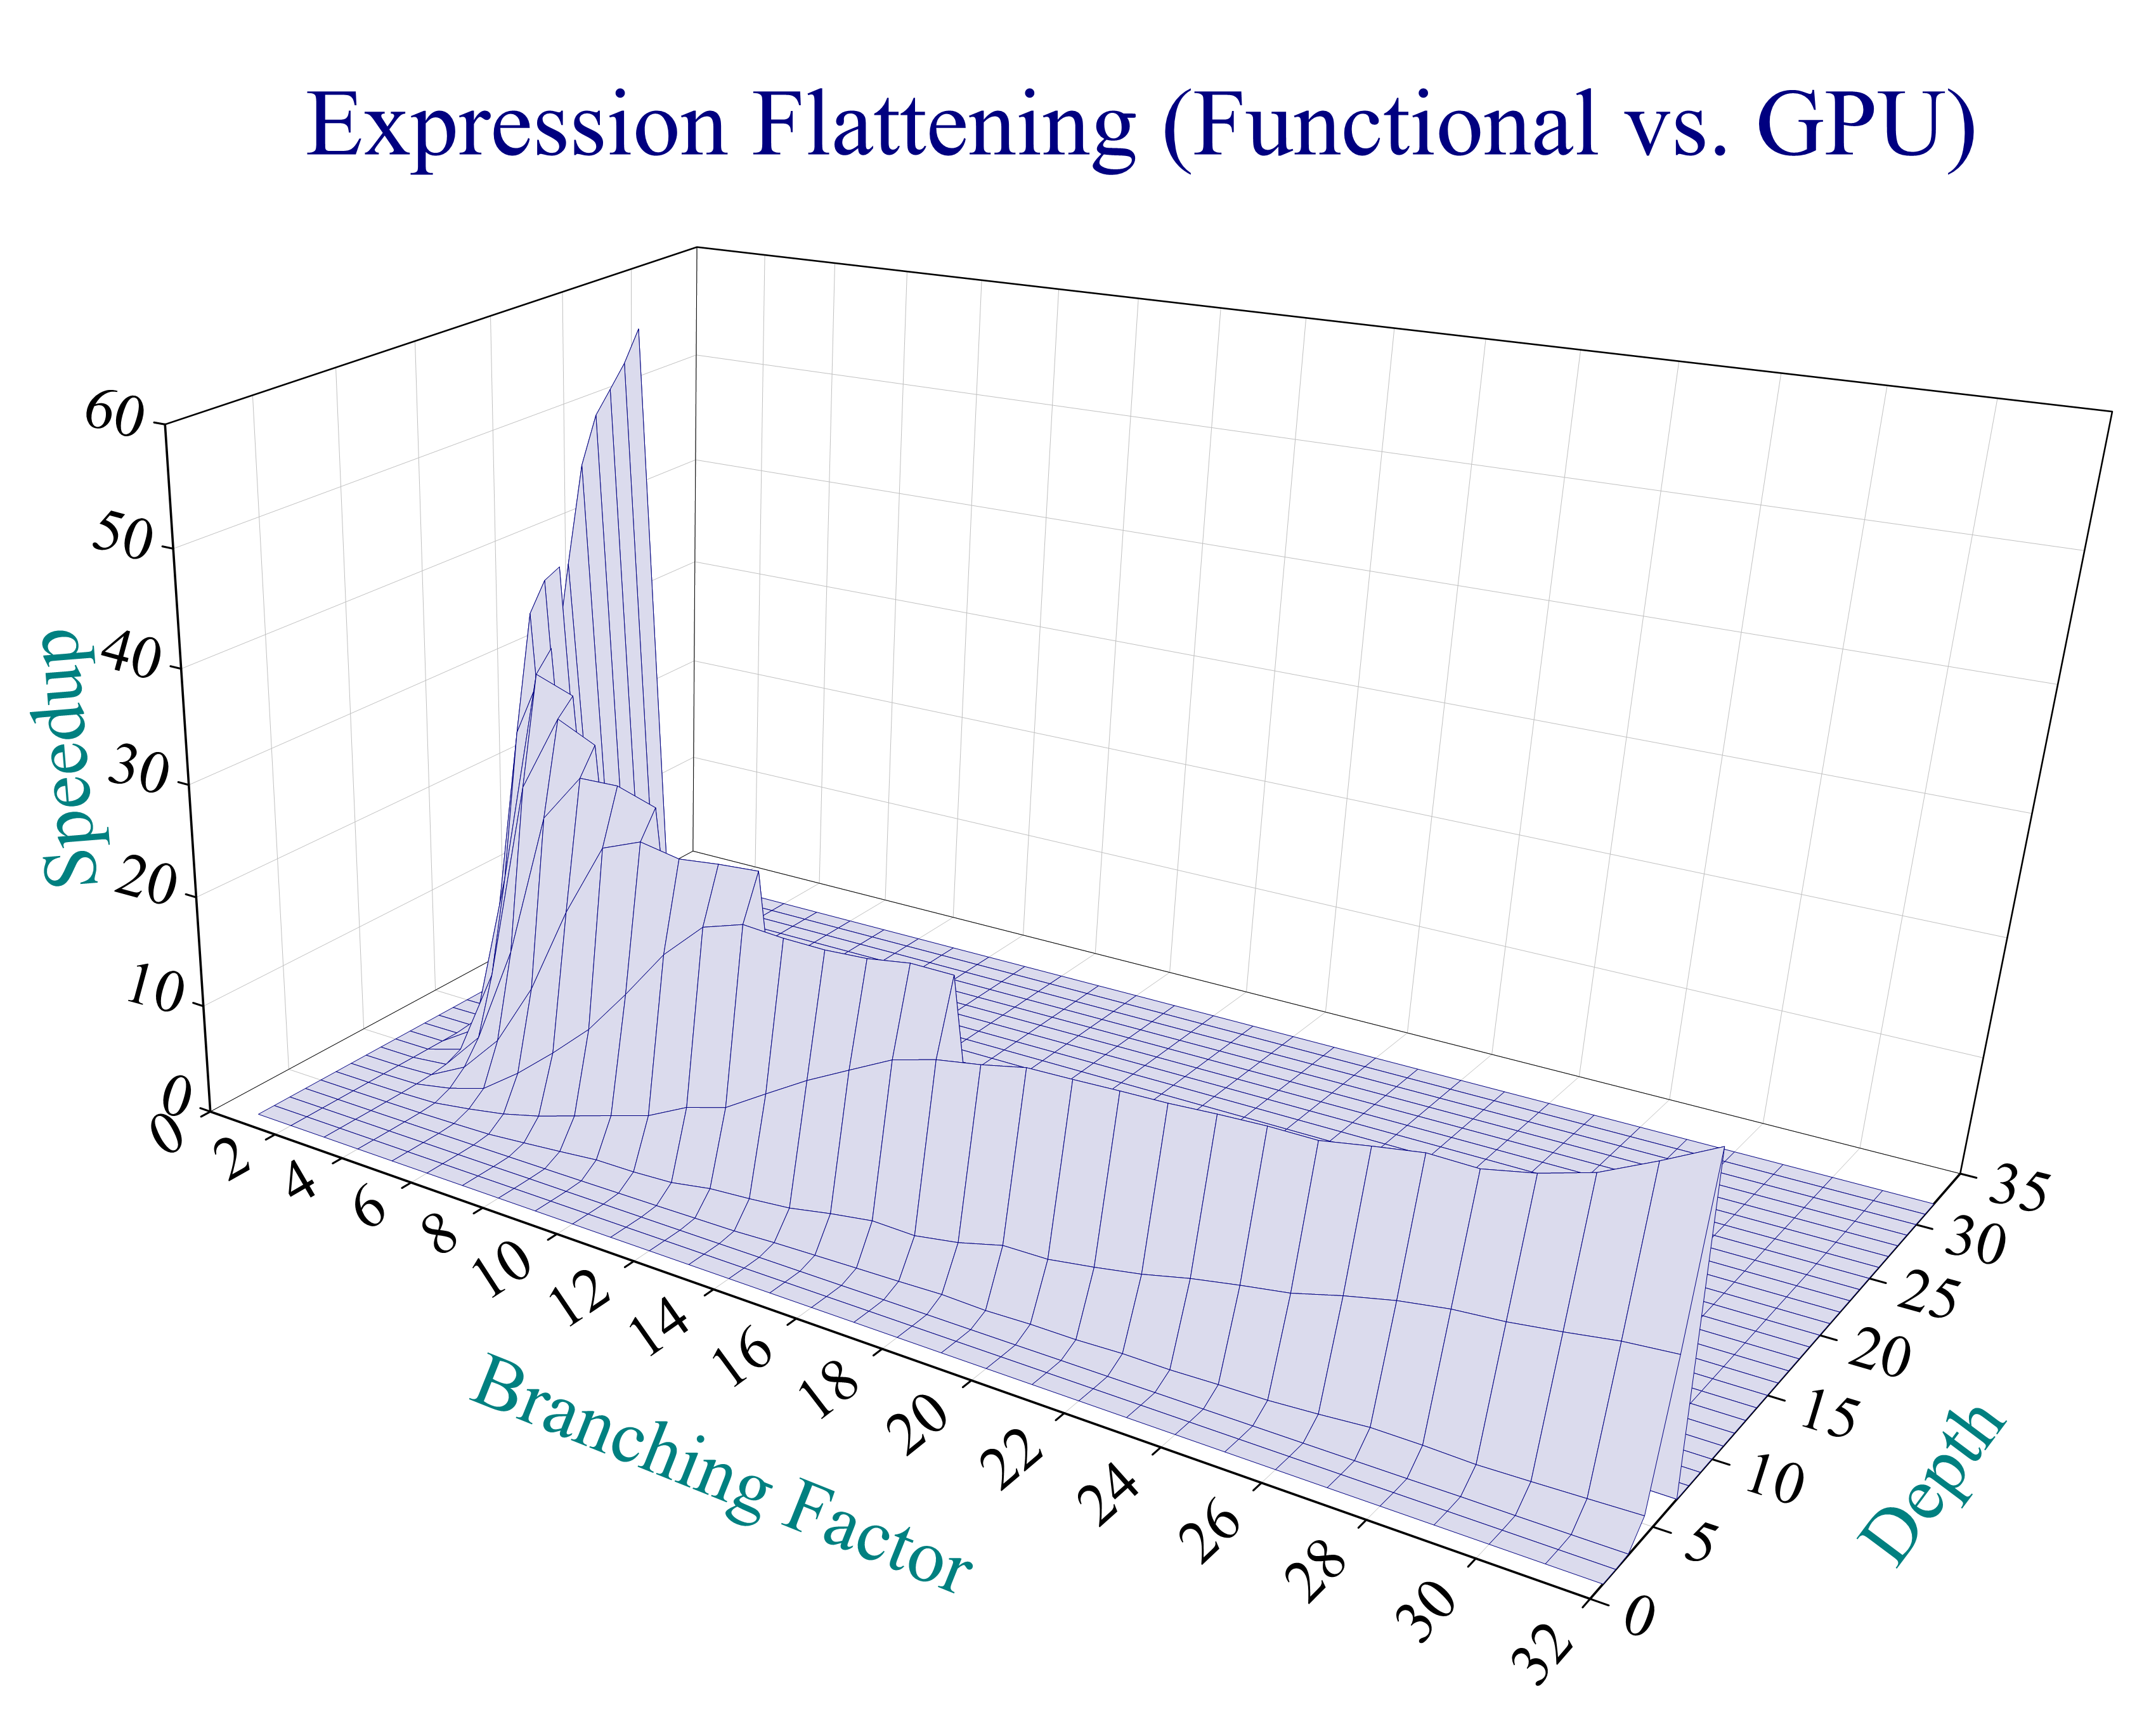
\includegraphics[width=3.3in]{fnc_gpu_3d}
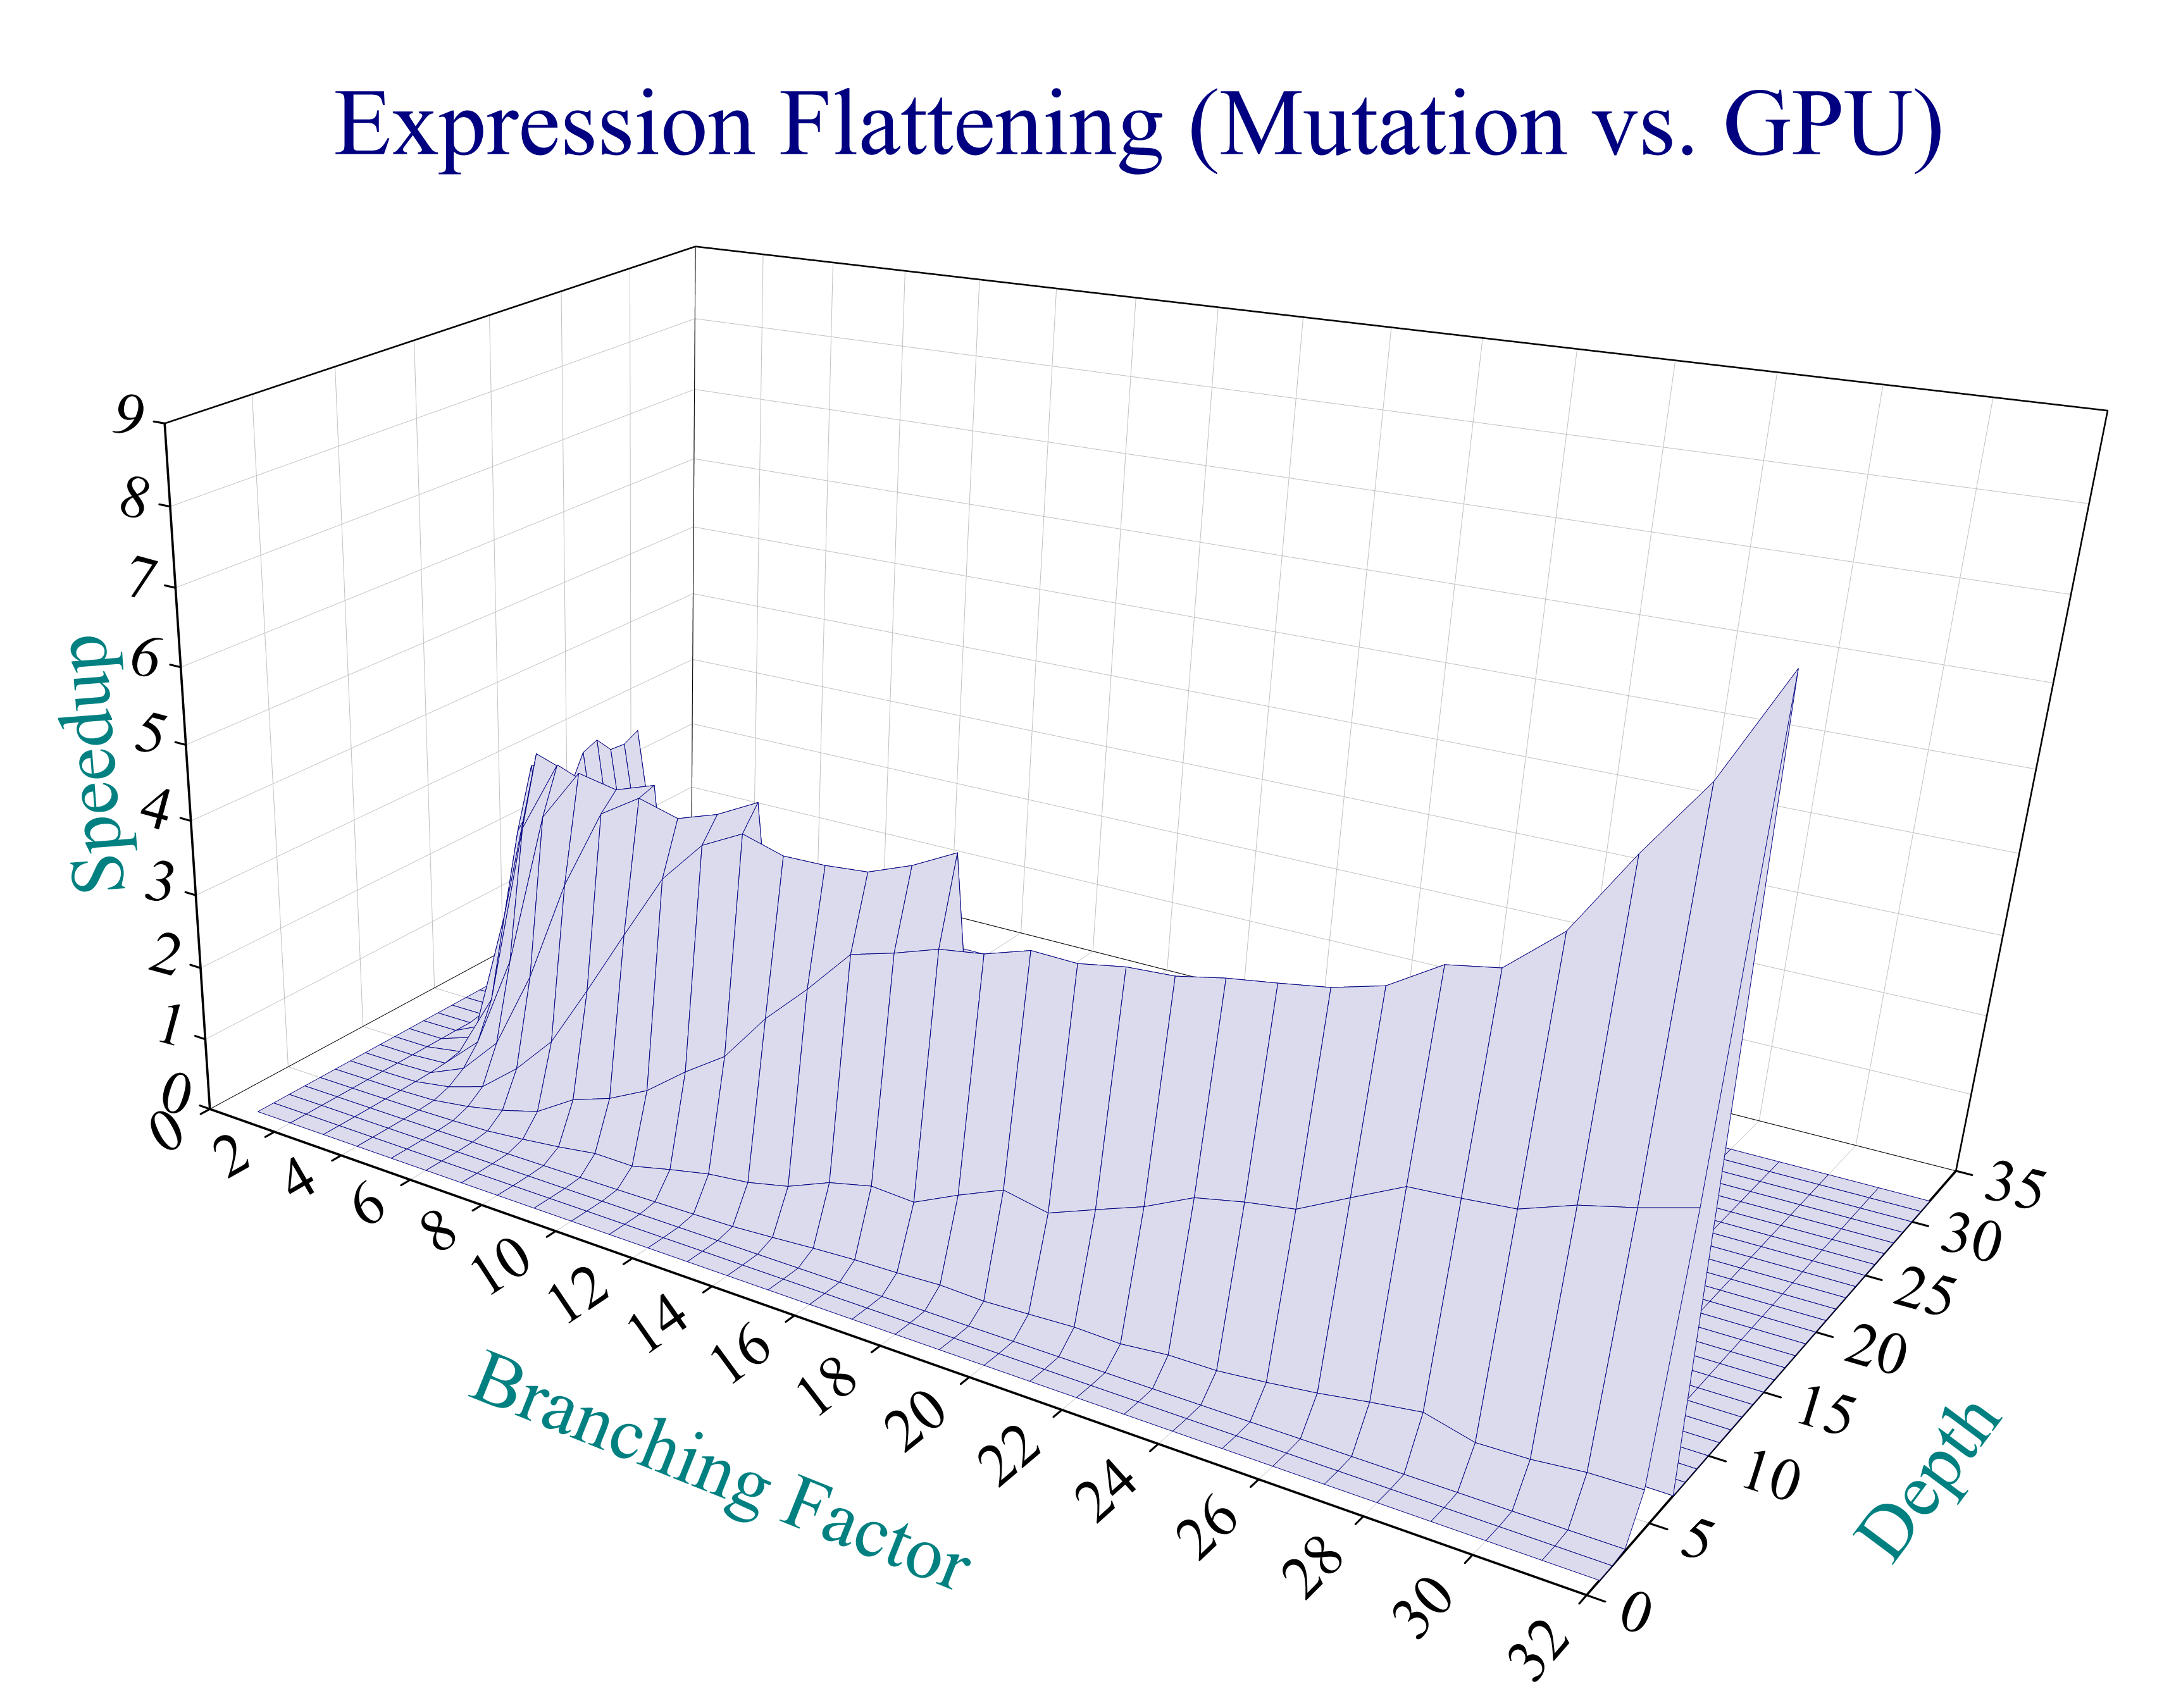
\includegraphics[width=3.3in]{mut_gpu_3d}
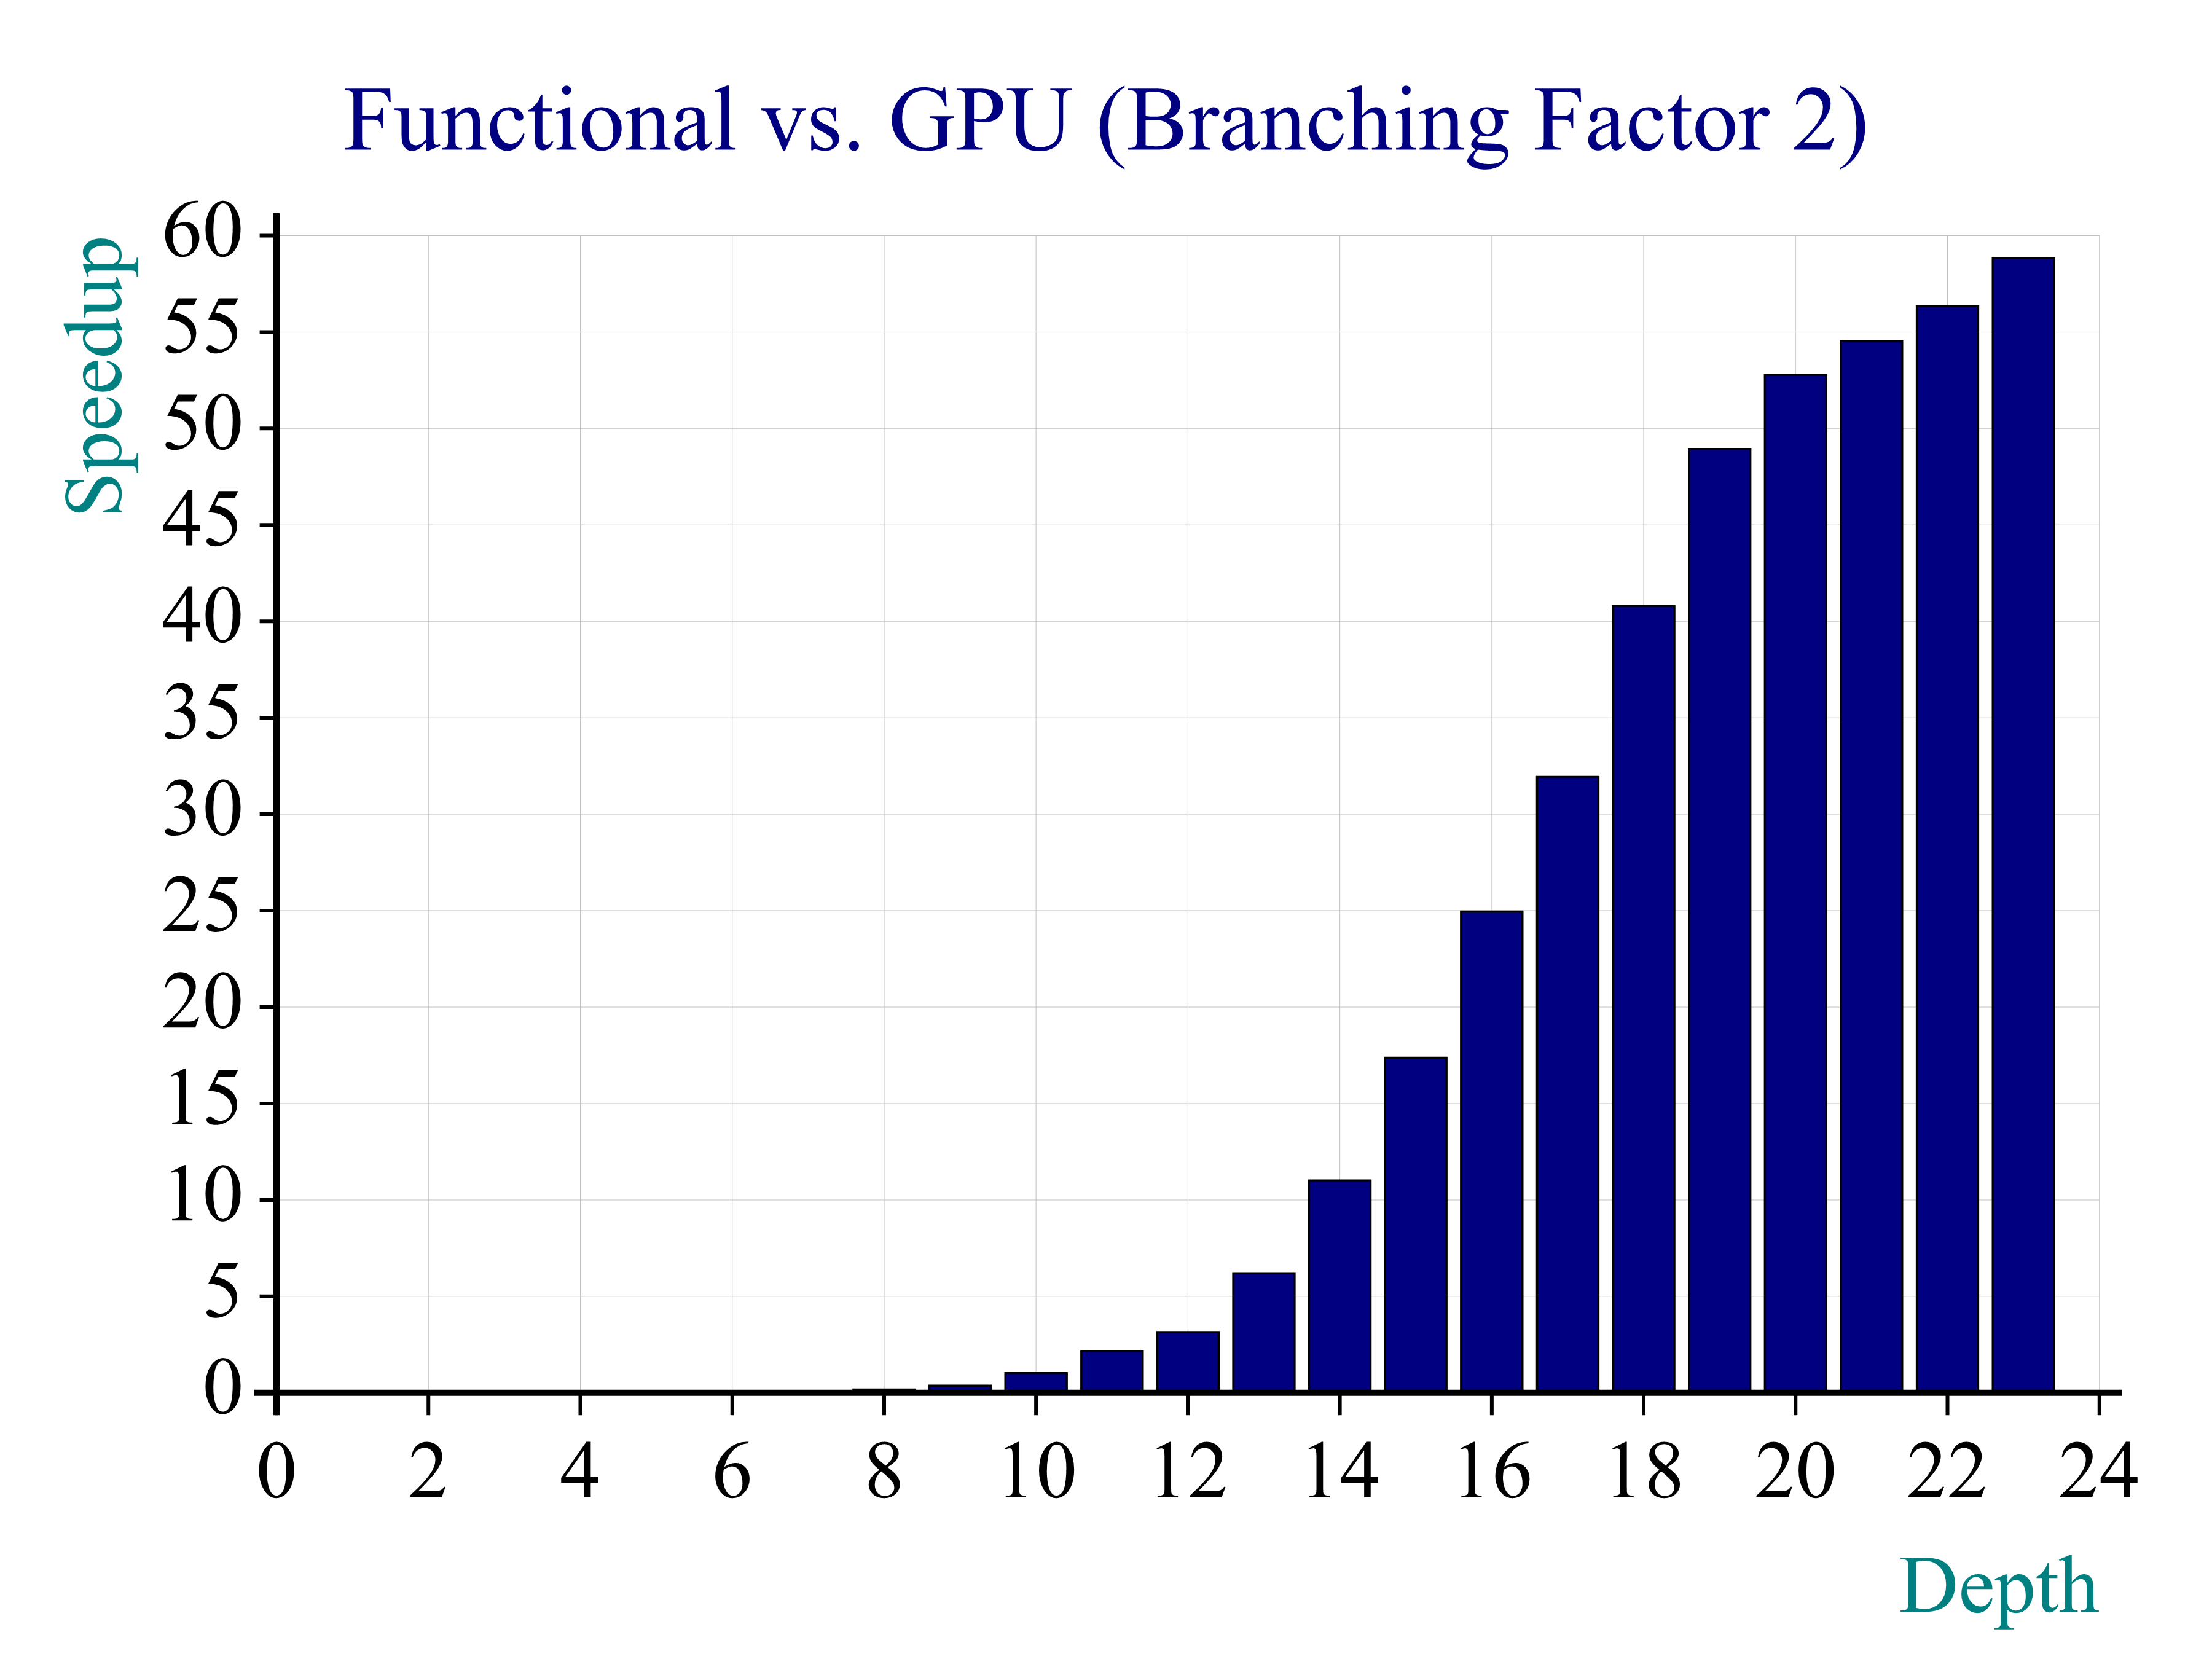
\includegraphics[width=3.3in]{fnc_gpu_2d}
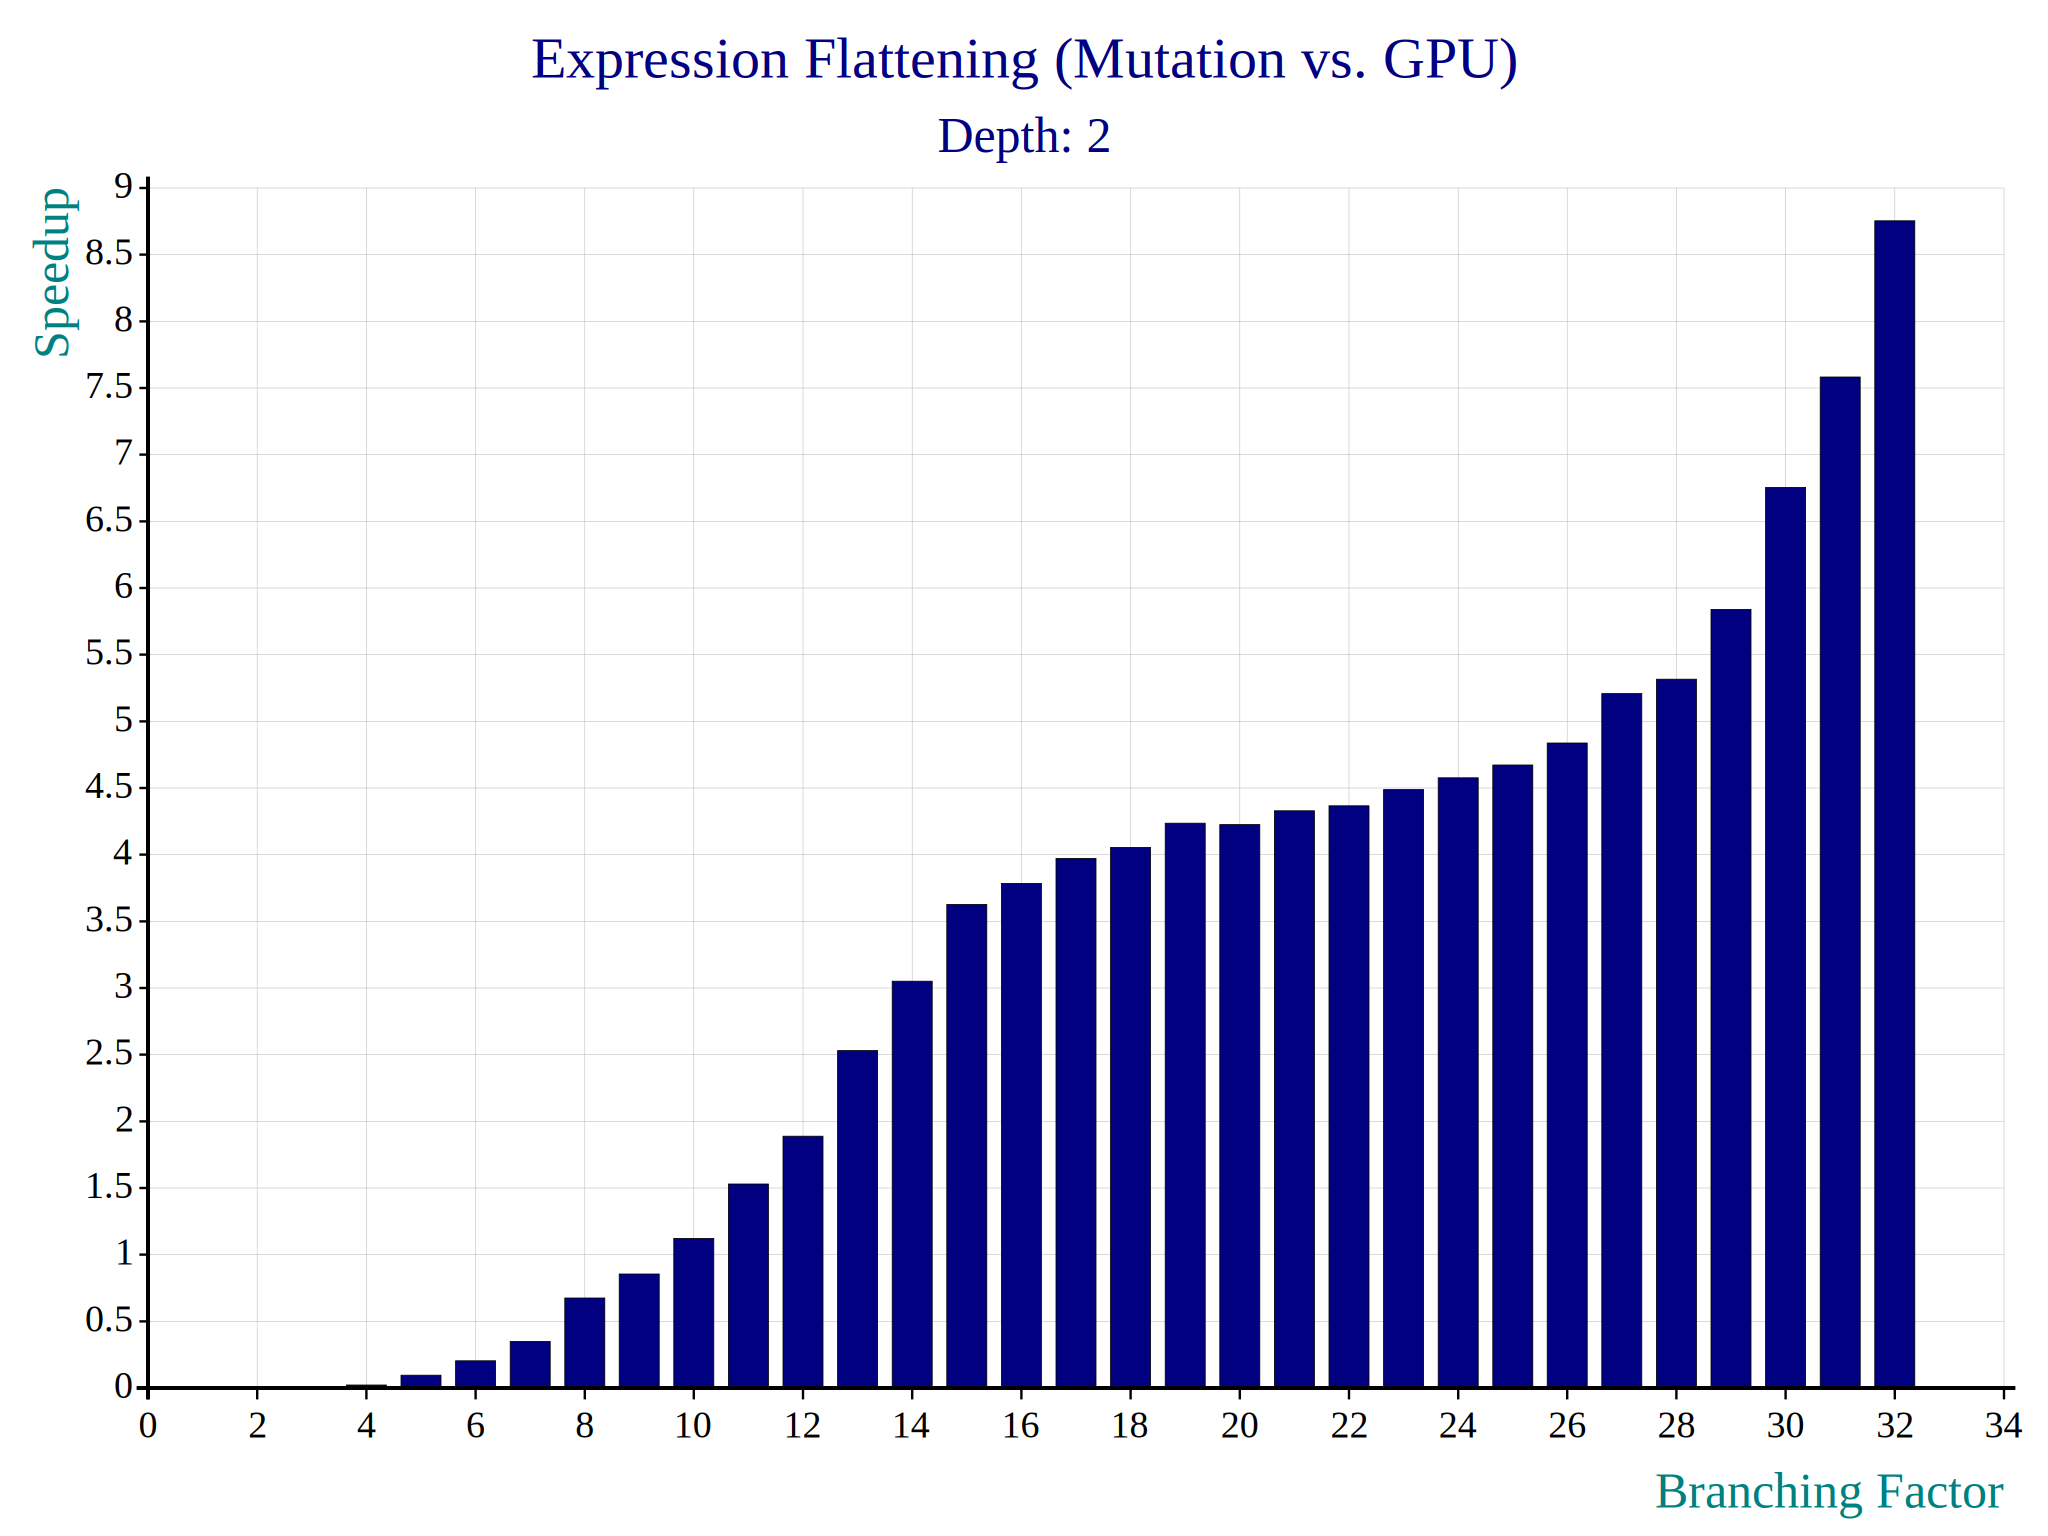
\includegraphics[width=3.3in]{mut_gpu_2d}
\end{center}
\caption{Performance of Key-based Expression Flattening compared to traditional methods}
\label{fig-bench}
\end{figure*}

\section{Performance}

To examine the performance characteristics of the above techniques, we prototyped a micro-benchmark that flattens expressions on an AST. This mimics the core functionality of both the function lifting and expression flattening passes described in more detail above and used in the Co-dfns compiler. It also serves to compare the performance of using Key (\verb;⌸;) based algorithms to perform tree transformation compared to recursively defined algorithms. We implemented the above lifting algorithm using CUDA 8.0 and Thrust primitives. 

We implemented the same algorithm using two traditional recursive methods. The first is a ``Functional'' analogue, that avoids mutation of the result and instead uses a pure-functional interface to pass nodes to be lifted back up the call stack. This is a very common method, taught in compiler courses that teach flattening passes, as well as used in various compilers. The benefit of the functional algorithm is the concision with which it may be written in most higher-level languages, particularly those which eschew mutatoin and favor a pure coding style. The disadvantage is that it has a higher memory usage requirement and may copy data as it moves up through the call stack to reassemble various containers for child nodes.

The second algorithm is a common optimization on the functional recursive style that makes use of an accumulator container that threads through the computation. The traversal functions will then mutate this accumulator as nodes are discovered that require lifting. The advantage over the functional method is that you can avoid excess copying overheads and in some languages that are more favorable to mutation, it may even be easier to write. A disadvantage is that you must be carefully aware of the order of traversal through the AST, since a change in the ordering of traversal can affect the order in which traversal functions write to the accumulator. This makes it less friendly to multi-threading. It can also be cumbersome or less desirable to write in this style in some programming languages in which the functional algorithm finds natural expression.

Normally, one would test GPU oriented benchmarks based on their input sizes. However, in this case, the traditional algorithms and the GPU algorithms are written quite differently. Thus, we introduce two dimensions of input size in order to examine differences with more precision. Particularly, we benchmarked the GPU algorithm against the traditional methods by depth of the AST and Branching Factor. We chose to examine depth as a specific factor because the path matrix is inherently dependent on the depth. Furthermore, the mutation algorithm is optimized in such a way that fewer expression nodes may result in fewer writes to the accumulator, while our algorithm has no such optimization, and traverses the entire tree independent of the number of expression nodes. 

We ran the benchmark to compute the time to flatten an AST on all combinations of depth and branching factor along the interval $[0,32)$ that were of a suitable size (that is, fit within the machine constraints). The GPU was an NVIDIA Tesla K40c, and the CPU was an Intel Xeon  E5-1620v3. 

Figure \ref{fig-bench} shows the results of this experiment. It is interesting to note the difference in shapes between the functional and mutation algorithms relative to the GPU algorithms when mapped along both the depth and branching factor. As expected, the speedups against the functional algorithm are higher on the whole because of the higher memory demands of that algorithm. All these algorithms should be memory bound, so a reduction in overall memory traffic benefits the mutation algorithm quite a bit. 

Our peak speedups are around 58× comparing against the functional algorithm, and around 9× when comparing against the mutation algorithm. However, the ``performance'' zone for the GPU algorithm is fairly similar in shape between the two. Particularly, this "curved mountain peak" represents the boundaries where the number of AST elements in the whole AST becomes large enough to attain sufficient parallelism on the GPU. 

The second row of graphs in Figure \ref{fig-bench} highlights a single plane of the mountain where we fix the branching factor or the depth. This gives a better picture of the behavior of the algorithm along the most pronounced areas of the area graph. These are also of particular interest because they represent two common cases found in real code. When the branching factor is 2, we have a reasonable analogue of common expressions found in code such as APL or other mathematically intense code which may have long strings of dense expressions, leading to a higher depth, but a low branching factor (since most operators of this sort take one or two arguments). When the Depth is fixed at 5, but we increase the branching factor, this more closely simulates code that may have functions nested throughout the code that need to be lifted which contain many child statements, but may not be particularly deep. In such cases the branching factor would increase, but the ASTs themselves may be relatively low depth. 

It should also be noted that while the mutation-oriented algorithm is obviously faster than the functional algorithm on the CPU, it comes at the cost of stylistic clarity and the capability to reason locally about computation. Our Key-based algorithm remains pure and functional while still being fast. It is also exceptionally concise relative to the other two algorithms.

\section{Discussion}

There are many options for representing graphs on data-parallel architecture. Most of them tend to optimize traversal instead of transformation. Because of the transformation heavy nature of compiler-style algorithms, these other representations can introduce work that complicates both the algorithms themselves, as well as the work necessary to maintain those structures over the lifetime of the compilation phase. 

The use of a path matrix provides benefits to locality, which allows for increased parallelism for transformation passes such as the flattening passes mentioned above. While this can be used to increase the performance of a single compiler pass, the above treatment is not intended primarily for highly optimizing a single pass in a compiler. Instead, the design of the above algorithms and techniques are designed to improve the data parallelism and ease of expression across the entire compiler, not just a single pass. 

To illustrate the difference, consider a few other possible representations. One possibility is the use of a single parent vector for the entire AST. We could also work directly off of the depth vector or the traditional method of listing pointers to the children and/or parents. In the case of the expression flattening above, we could likely achieve equal or better performance from using a single parent vector for this one computation. However, would be increasing costs elsewhere, particularly in maintenance. A path matrix provides both parent information, as well as information about the depth of the node, the siblings, position in the tree, and a unique identifier in a single structure that is cache/memory friendly. Since many operations on trees are memory bound, this memory optimization becomes important. In the Co-dfns compiler, we are able to generate the path matrix once, at the beginning of the compilation, and pass them around freely, and even duplicate them when appropriate, to communicate information without requiring cross thread or non-local memory access patterns.

This means that we never need to recompute the matrix, and indeed, doing so would defeat the purpose. In contrast, if you require a parent vector to organize your AST, then that parent vector may need to be shuffled, extended, and permuted each time the AST changes, and fails to maintain the original edge information of the graph. Keeping the original parent vector but maintaining a set of links would be a potential solution, but removes the locality of the access patterns, making it impossible to do a coalesced read of all of edge information needed for a single computation as a single access. Using a path matrix allows us to avoid that and increase the amount of stride-1 regular accesses and reduces memory indirections.

The cost of a path matrix is its size. Many other representations are size efficient, depending only on the number of nodes in the AST. A path matrix on the other hand, in the worst case, is dependent both on the depth of the AST and the number of nodes in the AST. Depending on the specific application, it is possible to choose different path matrix representations that optimize certain cases. For instance, one may not require that traversing the parent path be fast, and thus, we may reduce the cost of generating the path matrix by removing that requirement. Removing this requirement may also allow a path matrix to use a smaller sized integer representation for the matrix, further reducing the size at the cost of increased computation for certain operations. We have shown general path matrix techniques above that will work regardless of these particular choices in creating the path matrix. 

\section{Future Work}

The current compiler represents a non-trivial instance of the successful application of these techniques, but it focuses on an untyped, functionally oriented language. The type inference in the current version of the compiler is somewhat na\"ive. More work is required to expand the type inferencer to include more sophisticated type inference. The compiler does not currently handle errors such as signals or exceptions, nor does it implement some more sophisticated compiler optimizations. Further work remains to implement these techniques on an imperative and object-oriented language instead of a functional one. It would also be educational to implement a version for a lazy language.

We do not have a large scale understanding of the performance characteristics of these techniques in real life outside of daily use of the compiler. Further analysis is required to understand what sort of compiler optimizations and analyses are necessary to compile the Co-dfns compiler efficiently for the GPU and CPU. We currently lack a good comparison against existing techniques both for the compiler design and the generated code. Some existing compilers are able to compile variants of APL to target the GPU and the CPU, but there are subtle differences that require care when comparing generated code, and the architecture of these compilers is often quite different. Comparing the relative performance both of the compiler designs (human factors and execution speed) and generated code is important to understanding these techniques more fully.

While we have found this method of compiler construction to be very compact and to permit working with a data-parallel compiler as easily or nearly as easily as with a standard Nanopass compiler, we have not done extensive studies to determine just how comparable in programmability, ease of maintenance, or extensibility these techniques are with established compiler construction methods, such as OOP Visitors, Nanopass, or the type-directed functional style.

\section{Related Work}

Iverson introduced the idea of the Rank operator while at Sharp Associates \cite{iverson1983rationalized} as a part of ``Rationalized APL.'' The rank operator (\verb;⍤;) used here derived from the J language, a continuation of the rationalized APL idea, with many ideas such as rank percolating back into APL implementations. \cite{bernecky1987rank,hui1995rank} The J programming language \cite{hui2014key} was the first practical, general-purpose programming language to introduce the Key operator as a primitive operator with the presumption of its general usefulness.

Bernecky \cite{bernecky2015abstract} argues that the increased programmability and desirable human factors of APL-style array programming can be implemented with competitive performance relative to more traditional techniques. This suggests that programs written in this highly abstract style may not suffer the performance gap traditionally assumed to go with their desirable features. This work is bolstered by previous work on the high-performance implementation of array-oriented languages. \cite{ching1994experimental,ching1993primitive, ching1990automatic,ju1991exploitation, ju1991performance,bernecky1999reducing,schwarz1991acorn}

Fritz Henglein demonstrated a class of operations, called discriminators, of which the Key operator is a member \cite{henglein2013dd} , namely, a discriminator performs the same grouping computation as Key, but does not apply a function over these groups with their keys. Henglein provides a linear implementation of these operations.

The EigenCFA effort \cite{prabhu2011eigencfa} demonstrated significant performance improvements of a 0-CFA flow analysis by utilizing similar techniques to those demonstrated here. In particular, encoding the AST and using accessor functions have a very similar feel to the node coordinates and AST encoding given here, though they have a different formulation and spend considerable effort understanding the trade-offs of performance associated with the different encodings, whereas the encodings here were chosen for their clarity and directness, rather than their performance.

Mendez-Lojo, et al. implemented a GPU version of Inclusion-based Points-to Analysis \cite{mendez2012inclusion} that also focuses on adapting data structures and algorithms to efficiently execute on the GPU. In particular, they use similar techniques of prefix sums and sorts to achieve some of their adaptation to the GPU, Additionally, they have clever and efficient methods of representing graphs on the GPU which enable dynamic rewriting of the graph.

The APEX compiler \cite{bernecky1997apex} developed vectorized approaches to handling certain analyses to compile traditional APL, including a SIMD tokenizer \cite{bernecky2003tokenizer}. It also uses a matrix format to represent the AST. Traditional APL did not have nested function definitions, however, and thus the APEX compiler does not have any specific approaches to dealing with function lifting.

Timothy Budd implemented a compiler \cite{budd1984apl,budd2012apl} for APL which targeted vector processors as well as C. Budd provided thoughts and some ideas on how the compiler might be implemented in parallel as well.

J. D. Bunda and J. A. Gerth presented a method for doing table driven parsing of APL which suggested a parallel optimization for parsing, but did not elucidate the algorithm \cite{bunda1984apl}.

\section{Conclusion}

We have derived a method of performing computation over sub-trees selected on the basis of inter-node properties through the use of the Key (\verb;⌸;) operator and node coordinates, which enable local computation of these inter-node properties. This method is both general and direct, and when combined with traditional and more mundane array programming, suffices to implement the complete core of a compiler, modulo parsing and code generation. The method requires no special operations or unique special casing primitives in the language. Moreover, it is strictly data-parallel and data-flow, without any complex control flow, which results in exceptionally concise code. These methods permit a general, high-level approach to constructing a compiler that is parallel by construction by constricting the language to only a data parallel subset of a normal array language.

We have demonstrated the technique and the core insights behind the data structures involved. It presents a solution to a very old and traditional problem in a very uncommon light, by eschewing the common practices that underlie every other significant and general solution found in modern compilers today and replacing them with an entirely different paradigm centered on parallelism and aggregate operations. 
\balancecolumns

\bibliographystyle{abbrvnat}
\bibliography{biblio}

\begin{table*}
\centering
\begin{tabular}{cllcll}
\toprule
Symbol                   & Monadic            & Dyadic  &
Symbol                   & Monadic            & Dyadic  \\
\midrule
\multicolumn{6}{c}{Scalar Functions} \\ 
\midrule
\texttt{+}               & Identity           & Plus (Add) &
\texttt{\textasciitilde} & Not                & \\
\texttt{-}               & Negative           & Minus (Subtract) &
\texttt{?}               & Roll               & \\
\texttt{×}               & Direction (Signum) & Times (Multiply) &
\texttt{∧}               &                    & And \\
\texttt{÷}               & Reciprocal         & Divide &
\texttt{∨}               &                    & Or \\
\texttt{|}               & Magnitude          & Residue (Modulo) &
\texttt{⍲}               &                    & Nand \\
\texttt{⌊}               & Floor              & Minimum &
\texttt{⍱}               &                    & Nor \\
\texttt{⌈}               & Ceiling            & Maximum &
\texttt{<}               &                    & Less \\
\texttt{*}               & Exponential        & Power &
\texttt{≤}               &                    & Less Or Equal \\
\texttt{⍟}               & Natural Logarithm  & Logarithm &
\texttt{=}               &                    & Equal \\
\texttt{○}               & Pi Times           & Circular (Trigonometric) &
\texttt{≥}               &                    & Greater Or Equal \\
\texttt{!}               & Factorial          & Binomial &
\texttt{>}               &                    & Greater \\
\texttt{≠}               &                    & Not Equal \\
\midrule
\multicolumn{3}{c}{Selection Mixed Functions} &
\multicolumn{3}{c}{Structural Mixed Functions} \\
\cmidrule(r){1-3} \cmidrule(l){4-6}
\texttt{⊃}               & Disclose & Pick &
\texttt{⍴} & Reshape       & \\
\texttt{↑}               &          & Take &
\texttt{,} & Ravel         & Catenate/Laminate \\
\texttt{↓}               &          & Drop &
\texttt{⍪} & Table         & Catenate First/Laminate \\
\texttt{/}               &          & Replicate &
\texttt{⌽} & Reverse       & Rotate \\
\texttt{⌿}               &          & Replicate First &
\texttt{⊖} & Reverse First & Rotate First \\
\texttt{\textbackslash}  &          & Expand &
\texttt{⍉} & Transpose     & Transpose \\
\texttt{⍀}               &          & Expand First &
\texttt{↑} & Mix           & \\
\texttt{\textasciitilde} &          & Without (Excluding) &
\texttt{↓} & Split         & \\
\texttt{∩}               &          & Intersection &
\texttt{⊂} & Enclose       & Partitioned Enclose \\
\texttt{∪}               & Unique   & Union &
\texttt{∊} & Enlist        & \\
\texttt{⊣}               & Same     & Left \\
\texttt{⊢}               & Identity & Right\\
\midrule
\multicolumn{3}{c}{Selector Mixed Functions} &
\multicolumn{3}{c}{Miscellaneous Mixed Functions} \\
\cmidrule(r){1-3} \cmidrule(l){4-6}
\texttt{⍳} & Index Generator & Index Of &
\texttt{⍴} & Shape         & \\
\texttt{∊} &                 & Membership &
\texttt{≡} & Depth         & Match \\
\texttt{⍋} & Grade Up        & Grade Up &
\texttt{≢} & Tally         & Not Match \\
\texttt{⍒} & Grade Down      & Grade Down &
\texttt{⍎} & Execute       & Execute \\
\texttt{?} &                 & Deal &
\texttt{⍕} & Format        & Format \\
\texttt{⍷} &                 & Find &
\texttt{⊥} &               & Decode (Base) \\
& & & \texttt{⊤} &               & Encode (Representation) \\
& & & \texttt{⌹} & Matrix Divide & Matrix Inverse \\
\end{tabular}
\caption{Primitive Functions}
\label{tab:scalarprims}
\end{table*}

\begin{table*}
\centering
\begin{tabular}{cll}
\toprule
Symbol     & Name & Description \\
\midrule
\texttt{⍨} & Commute & Swaps arguments or distributes
 right argument to both sides \\
\texttt{¨} & Each & Applies its operand point-wise over the left/right
 arguments \\
\texttt{/} & Reduce & Reduce along the last axis \\
\texttt{⌿} & Reduce First & Reduce along the first axis \\
\texttt{\textbackslash} & Scan & Scan along the last axis \\
\texttt{⍀} & Scan First & Scan along the first axis \\
\texttt{⌸} & Key & Apply operand once for each sub-array grouped by key \\
\end{tabular}
\caption{Primitive Monadic/Unary Operators, each takes a single left
operand and describes a function operating over one or two arguments}
\label{tab:adverbs}
\end{table*}

\begin{table*}
\centering
\begin{tabular}{cll}
\toprule
Symbol     & Name & Description \\
\midrule
\texttt{∘} & Compose & Composes two operands as in traditional mathematics \\
\texttt{.} & Inner Product & Inner product operation, e.g.
 \texttt{+.×} for matrix multiplication \\
\texttt{∘.} & Outer Product & Cartesian product or ``function table'' \\
\texttt{⍣} & Power & Iteration, Limited use only \\
\texttt{⍤} & Rank & Apply a function along cells of an array \\
\end{tabular}
\caption{Primitive Dyadic/Binary Operators, each takes a left
 and right operand and describes a function operating over one or two arguments}
\label{tab:conjunctions}
\end{table*}

\end{document}
